The experiments consists of three sub experiments. In the first, baseline, experiment default evolutionary policy search is tested on the toy problem defined in section \ref{toyprob}. In the second experiment the effect of co-evolution is tested in order to validate the reduction of sample complexity and, thirdly, in the third experiment GP CEPS is applied. Lastly in order to anaalyze the certainty of the gaussian process, the predicted mean, upper bound and lower bound is examined when applying GP CEPS on the toy problem.

\subsection{Evolutionary Policy Search}

In the evolutionary policy search approach the policies were restricted to those with 4 hidden units, and the parameters are as defined in section \ref{evo_pol_search}. Figure \ref{Fitness during Evolutionary Algorithm} is the average result of ten runs. The x-axis shows the amount of epochs (evoluations), and the y-axis represents the return of the best performing policy in the pool where 95\% confidence intervals are shown. For each epoch five evaluations are done per organism, and the pool size is 20. The performance on x-axis $30$ thus required $30 \times 5 \times 20$ samples. % TODO: ugly last sentence??

\begin{figure}[ht]
  \centering
  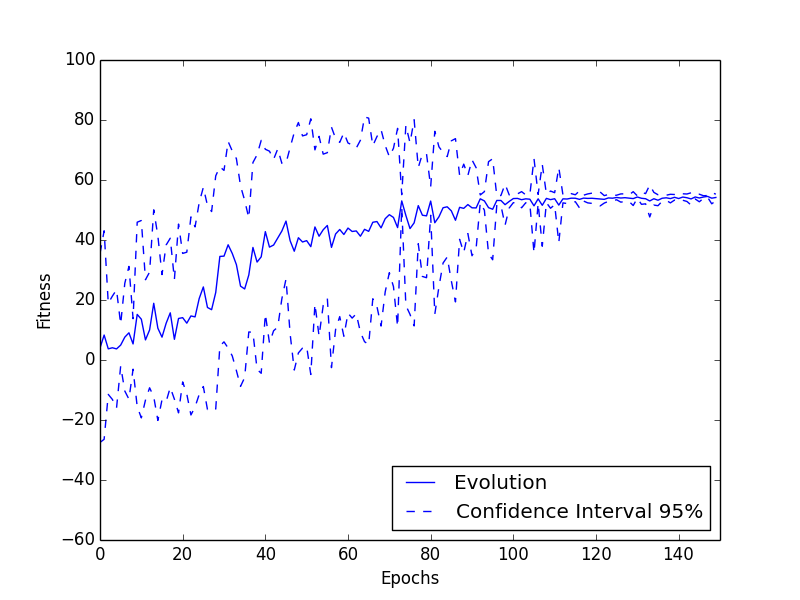
\includegraphics[scale=0.5]{images/evo.png}
  \caption{Fitness during Evolutionary Algorithm}\label{Fitness during Evolutionary Algorithm}
\end{figure}

Figure \ref{Example policy learned with evolutionary algorithm} shows the behavior of an example policy found with the evolutionary policy search algorithm, after 200 epochs. The wind is sampled from a uniform distribution between 0 and 0.5. Note that for all wind strengths, this policy reaches the goal. 

\begin{figure}[ht]
  \centering
  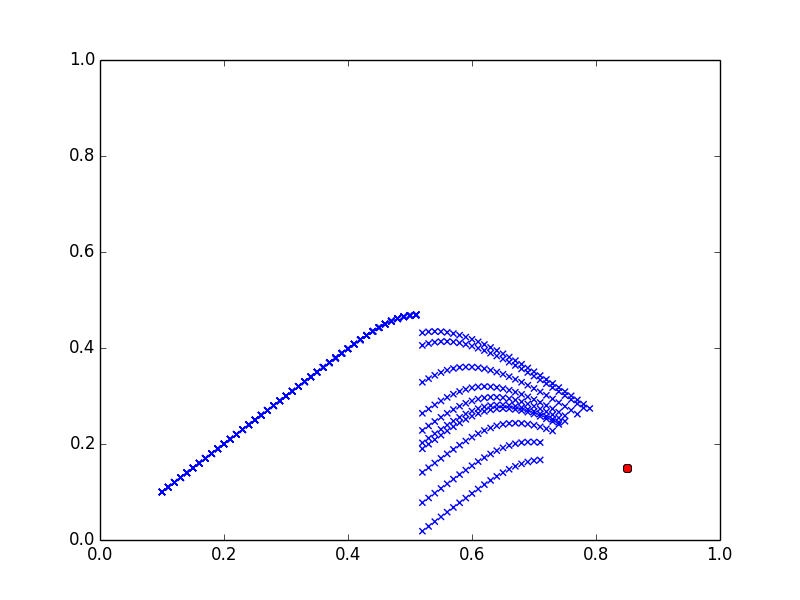
\includegraphics[scale=0.5]{images/evo_result.png}
  \caption{Example policy learned with evolutionary algorithm}\label{Example policy learned with evolutionary algorithm}
\end{figure}

\subsection{Co-Evolutionary Policy Search}

The results for Co-Evolutionary Policy Search are shown in Figure \ref{Fitness during Co-Evolutionary Algorithm}. 

\begin{figure}[ht]
  \centering
  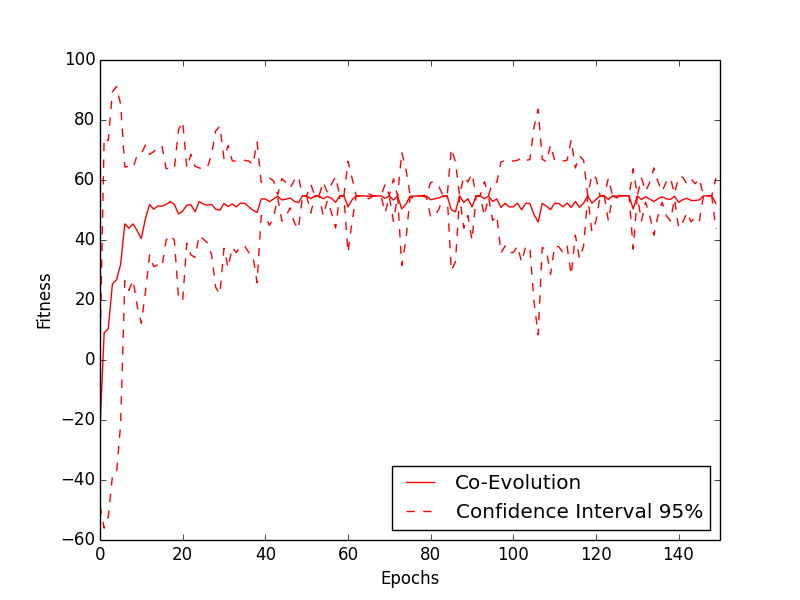
\includegraphics[scale=0.5]{images/co_evo.png}
  \caption{Fitness during Co-Evolutionary Algorithm}\label{Fitness during Co-Evolutionary Algorithm}
\end{figure}

Once again, an MLP with 4 hidden units was trained, and the same general evolutionary parameters from section \ref{evo_pol_search} were used. An example policy trained with Co-Evolutionary Policy Search for 200 epochs is visualized in Figure \ref{Example policy learned with Co-Evolutionary algorithm}. This policy, too, is able to reach the goal for any wind strength. The same sample complexity as in the first experiment applies.


\begin{figure}[ht]
  \centering
  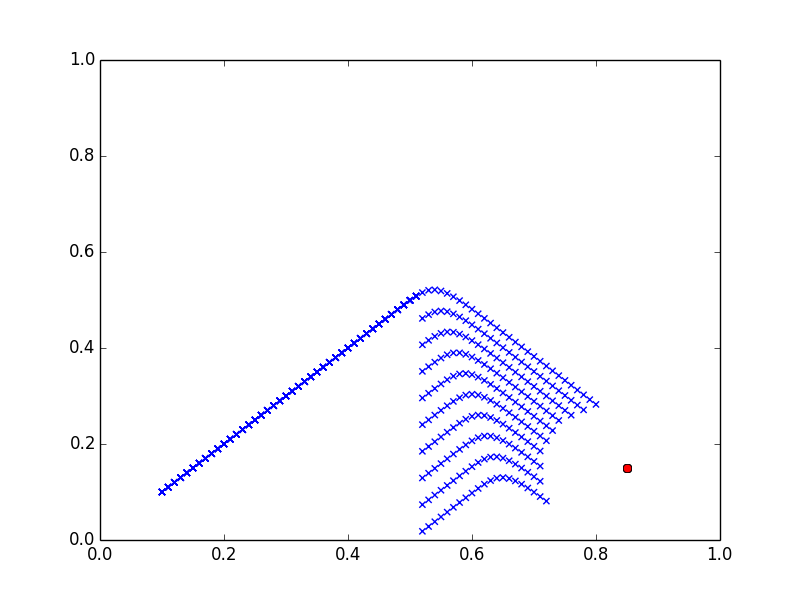
\includegraphics[scale=0.5]{images/co_evo_result.png}
  \caption{Example policy learned with Co-Evolutionary algorithm}\label{Example policy learned with Co-Evolutionary algorithm}
\end{figure}

\subsection{GP CEPS}

In this experiment we apply GP CEPS to the same problem, restricting to policies with 4 hidden units. Figure \ref{Example policy learned with GP CEPS} shows the fitness of the policy found using the primary optimization problem. The x-axis denotes the amount of samples taken from the real world (so $x=200$ means $200$ samples). 

% requires proper path
%\begin{figure}[ht%]
  %\centering
  %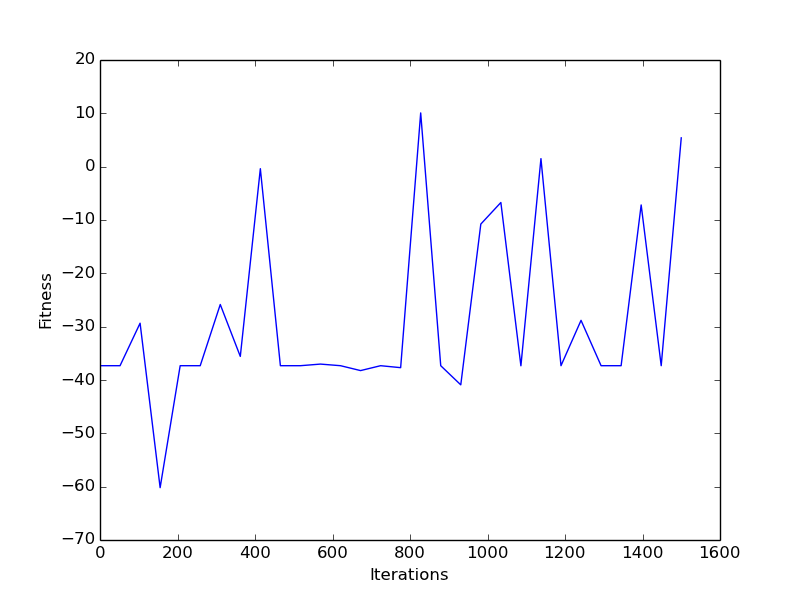
\includegraphics[scale=0.5]{images/GPCEPS_True.png}
  %\caption{Fitness during GP CEPS}\label{Fitness during GP CEPS}
%\end{figure}

% TODO: more info?
In addition the predicted mean, upper confidence bound (UCB) and $lower confidence bound$ (LCB) is shown in figure \ref{Fitness during GP CEPS}. 

%\begin{figure}[ht]
  %\centering
  %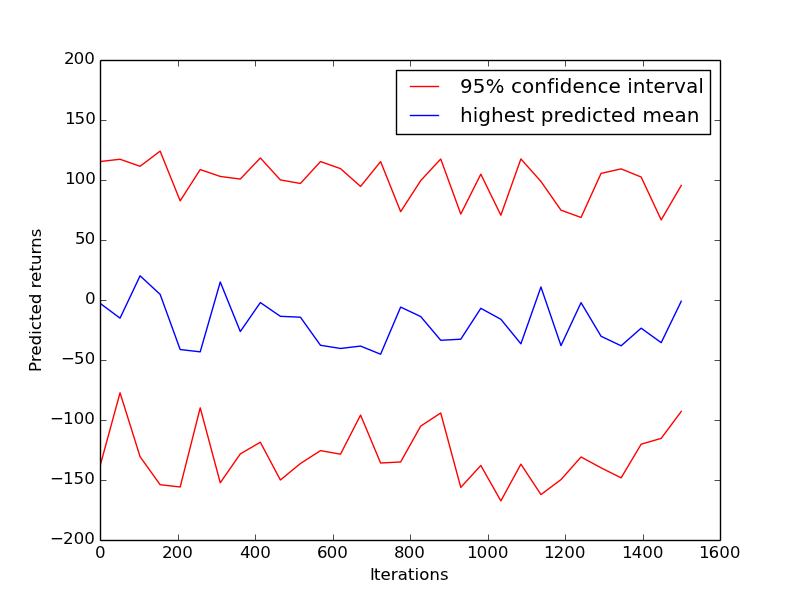
\includegraphics[scale=0.5]{images/GPCEPS_pred.png}
  %\caption{Predicted mean, UCB and LCB during GP CEPS}\label{Fitness during GP CEPS}
%\end{figure}


\subsection{Comparison}
In order to better compare the two evolutionary methods (without a GP) their results are shown together in figure \ref{compare_img}. It shows co-evulution leads to a steeper learning rate, whereas all policies of both methods eventually reach the target.

%\begin{figure}[ht]
  %\centering
  %\includegraphics[scale=0.5]{images/compare.png}
  %\caption{Comparing the performance normal and co-Evulationary algorithms in required samples}\label{compare_img}
%\end{figure}


